\documentclass[11pt]{article}
\usepackage{amsmath,amsthm,amssymb}
\usepackage{graphicx}
\usepackage{fontspec}
\setmainfont{Arial}
\usepackage{wrapfig}
\usepackage[toc,page]{appendix}
\usepackage[font=footnotesize]{caption}
\usepackage[margin=0.5in]{geometry}
\usepackage[singlespacing]{setspace}
\usepackage[small, compact]{titlesec}  % http://ctan.mirrors.hoobly.com/macros/latex/contrib/titlesec/titlesec.pdf
\titleformat*{\subsubsection}{\slshape}
\usepackage{paralist}
\renewenvironment{thebibliography}[1]{
    \let\par\relax\let\newblock\relax
    \inparaenum[\bfseries{[}1{]}]}{\endinparaenum}
\usepackage[english]{babel}
\pagenumbering{gobble}
\usepackage{lineno}
%\linenumbers % remove before submitting

\begin{document} % 7 page limit
\sloppy
\begin{center}
\large{\textbf{
    Functional Activity of the Human Gut Microbiome to Classify Colorectal Cancer
}} \\
\vspace{11pt}
\small{
    Kelly L. Sovacool \\
    August 2020
}
\end{center}

\section*{Specific Aims} % 1 page

Changes in the taxonomic composition and metabolic activity of human microbiomes have been observed in several diseases.
In the case of colorectal cancer (CRC), evidence of toxigenic activity by gut microbes implies that these changes are not only a response to disease, but may also play a role in disease etiology.
Taxonomic composition is commonly defined by amplicon sequencing of the 16S rRNA gene and clustering sequences into Operational Taxonomic Units (OTUs).
Previous studies have built OTU-based machine learning models to classify stool samples as normal or cancerous, to serve as a less invasive diagnostic tool for CRC than colonoscopy.
Efforts to find consistent changes in taxonomic composition of microbiomes between normal and dysbiotic states have found mixed success, in part because interpersonal variability in taxonomic composition sometimes exceeds the variability between disease states.
Variability of microbiome composition between individuals with the same disease status may be explained by functional redundancy, where different microbial species carry out the same functions and thus can replace each other with little effect on the overall function of the community.

Sequencing whole metagenomes to identify the genes present and annotate known gene functions is commonly used to build a profile of functional potential of the microbiome.
Combining taxonomic composition from OTUs with functional potential from metagenomes allows one to characterize functional redundancy across communities, where communities with similar functional potential have different taxonomic composition.
Untargeted mass spectrometry can validate the functional potential characterized from metagenomics by identifying metabolites that are active in a community, thus painting a more precise picture of active microbial functions.
Here, I propose to investigate the impacts of taking functional redundancy and active metabolites into account on human stool sample classification for CRC diagnosis.

\subsection*{Aim 1. Assess the impact of functional redundancy of the gut microbiome on CRC classification.}
\textit{Hypothesis: Using functional gene profiles instead of only taxonomic profiles improves the classification modeling of samples as CRC or non-cancerous because of functional redundancy in the gut microbiome.}
\begin{compactenum}[A.]
    \item Build taxonomic profiles with OTUs from 16S rRNA gene sequences and build profiles of functional gene potential from metagenomes.
    \item Compare taxonomic composition to functional gene potential of microbiomes within and between disease states to determine presence and degree of functional redundancy.
    \item Build machine learning models to classify samples as CRC or non-cancerous with taxonomic composition, functional gene potential profiles, or both as model features and compare performance.
\end{compactenum}

\subsection*{Aim 2. Assess the impact of integrating active metabolites with functional gene potential on CRC classification.}
\textit{Hypothesis: Using active metabolic pathways confirmed with mass spectrometry instead of all potential metabolic pathways from metagenomes improves the classification modeling of samples as CRC or non-cancerous.}
\begin{compactenum}[A.]
    \item Annotate compounds from untargeted mass spectrometry with the GNPS database and select those known to be products of bacterial metabolic pathways with the MetaCyc database.
    \item Calculate the intersection of pathways associated with active metabolites and the pathways from functional potential profiles from metagenomes.
    \item Build machine learning models to classify samples as CRC or non-cancerous with all potential metabolic pathways or only confirmed active metabolic pathways as model features and compare performance.
\end{compactenum}

\section*{Dataset}
Stool samples were collected from patients undergoing colonoscopy as part of the GLNE 007 study (https://clinicaltrials.gov/ct2/show/study/NCT00843375).
211 individuals were diagnosed with CRC and 223 were confirmed non-cancerous.
16S rRNA gene amplicon sequencing was performed and remaining stool was kept frozen.
Part of the remaining stool will be used for whole metagenome shotgun sequencing and untargeted tandem mass spectrometry to complete these aims.

\section*{Background and Motivation} % 1/2 - 1 page

genetics and environmental factors explain only a small proportion of disease incidence, so we turn to the microbiome \cite{thomas_metagenomic_2019}.

``it is not possible to classify individuals as having healthy colons or screen relevant neoplasia using Bray- Curtis distances based on the 16S rRNA gene sequences collected from fecal samples (see Fig. S1 in the supplemental material). This variation is likely due to the ability of many bacterial populations to fill the same niche such that different populations cause the same disease in different individuals. Furthermore, a growing number of studies have shown that it is rare for a single bacterial species to be associated with a disease. Instead, subsets of the microbiome account for differences in health.'' \cite{topcuoglu_framework_2020} (Fig. \ref{fig:nmds_otu})

\begin{wrapfigure}{R}{0.5\textwidth}
    \begin{center}
        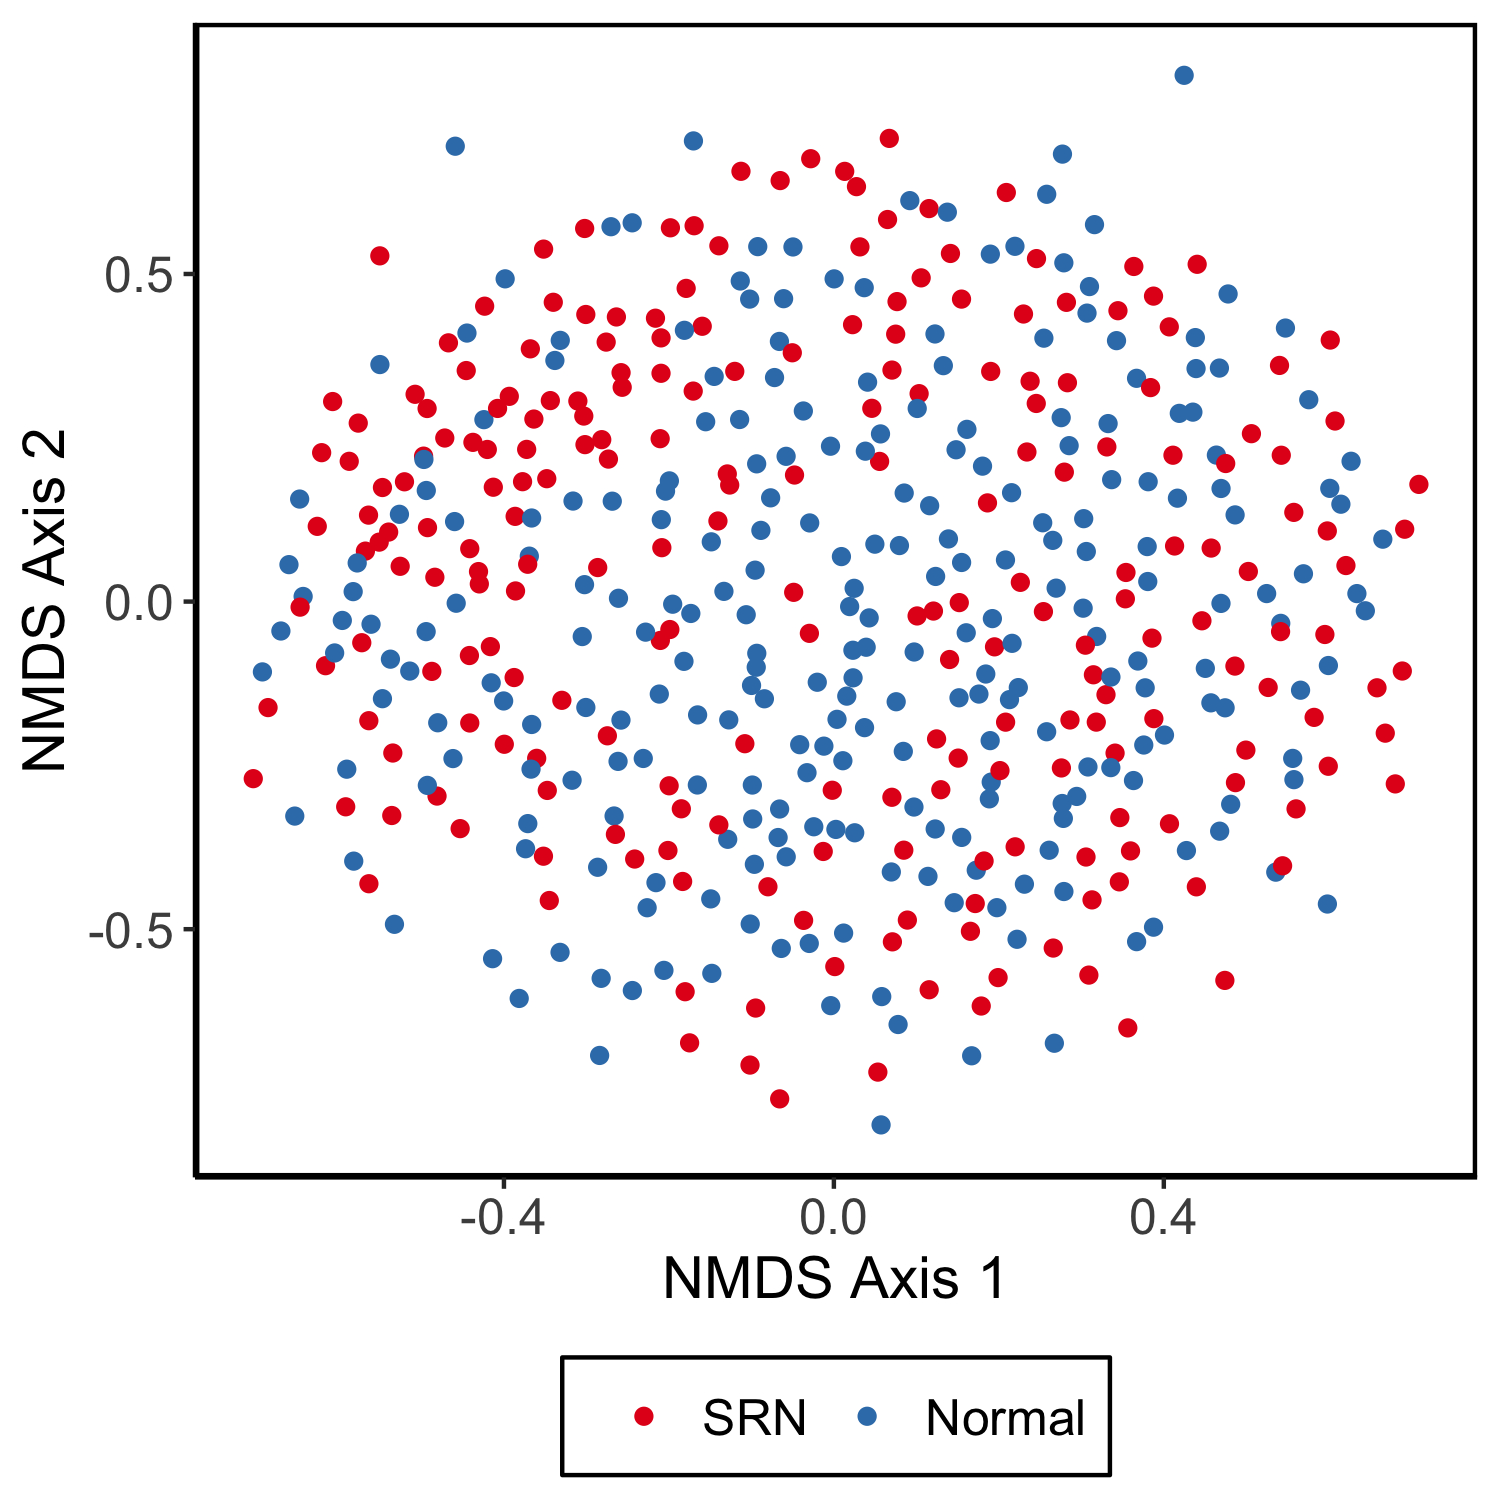
\includegraphics[width=0.5\textwidth]{figures/topcuoglu_s1.png}
        \caption{``Nonmetric multidimensional scaling (NMDS) ordination of Bray-Curtis distances. NMDS ordination relating the community structures of the fecal microbiota from 490 patients (261 patients with normal colonoscopies and 229 patients who have screen relevant neoplasias [SRNs]).'' \cite{topcuoglu_framework_2020}}
        \label{fig:nmds_otu}
    \end{center}
\end{wrapfigure}

other studies found specifical potential functional pathways that are CRC biomarkers, especially choline metabolism pathway \cite{thomas_metagenomic_2019}.


we don't know enough about functional redundancy in the human gut microbiome \cite{heintz-buschart_human_2018}

``Community-level function is often more conserved than community composition15,39–41, con- sistent with a functional repertoire ‘defining’ a niche and satisfied by different microbial assemblages.'' \cite{franzosa_species-level_2018}

many published studies claiming to have found functional redundancies in microbial systems lack quantitative analyses of redundancy \cite{souza_metagenomic_2015, ferrer_microbiota_2013}.

no one agrees on exact definition of functional redundancy \cite{louca_function_2018, heintz-buschart_human_2018, tully_dynamic_2018, royalty_quantitative_2020}.
``Stability in ecosystem function with increasing microbial diversity is often considered an empirical indication of functional redundancy''
\cite{royalty_quantitative_2020}


trait contribution evenness (TCE): ``the evenness in relative contribution of that trait among taxa within the community... This definition has several appealing properties including: TCE is an extension of established diversity theory, functional redundancy measurements from communities with different richness and relative trait contribution by taxa are easily comparable, and any quantifiable trait data (genes copies, protein abundance, transcript copies, respiration rates, etc.) is suitable for analysis.'' \cite{royalty_quantitative_2020}

``Functional redundancy is a measure of the number of different populations within a community that are able to perform the same functions. Functional redundancy can increase functional resilience, in case perturbations affect the taxonomic community structure; this allows for a return to community function, and therefore can increase stability.'' \cite{heintz-buschart_human_2018}

``This functional redundancy is further reflected in the fraction of the observed microbial community capable of participating in each metabolic step, with no statistically significant difference between the boreholes, except for ammonia oxidation (Figure 6).'' (used Student's t-test and Wilcoxon rank sum) \cite{tully_dynamic_2018}

\section*{Significance} % 1/2 page


\section*{Research Design and Methods}

\subsection*{Aim 1. Functional redundancy of the gut microbiome}

\paragraph{1A) Build profiles of taxonomic composition and functional potential.}

16S rRNA gene sequencing was previously performed on stool samples from patients in the GLNE 007 cohort for classification modeling to detect CRC \cite{baxter_microbiota-based_2016}.
Since then, additional samples have been collected and sequenced, bringing the total dataset to 211 CRC and 223 non-cancerous samples.
Sequences will be processed with mothur according to the MiSeq SOP \cite{schloss_introducing_2009, kozich_development_2013}.
Briefly, processing steps include filtering for quality, removing chimeric sequences, clustering sequences into OTUs using the \textit{de novo} OptiClust method with a similarity threshold of 97\%,
and generating a table of OTU abundances by samples \cite{westcott_opticlust_2017}.
Abundances will be rarefied and converted to relative abundances to circumvent biases in sampling depth across samples.
This final OTU abundance table will serve as the taxonomic composition profiles of each community.

Whole metagenome shotgun sequencing will be performed and metagenomes will be processed with HUMAnN2 \cite{franzosa_species-level_2018} to characterize functional potential of the CRC and non-cancerous microbial communities.
Sequences will be filtered and trimmed for quality prior to processing with HUMAnN2.
HUMAnN2 uses MetaPhlan2 to screen sequences against a curated reference of 400,000 clade-specific marker genes to detect the microbial species present in each sample \cite{segata_metagenomic_2012}.
This strategy is assembly-free and saves considerable computational resources over assembly-based methods.
Next, sequences are mapped to annotated reference genomes to identify the gene families defined by Uniref90 and the metabolic pathways defined by MetaCyc \cite{capsi_metacyc_2018} that are encoded by each community.
The MetaCyc database contains pathways involving both primary and secondary metabolism and can be filtered by the domain of life.
MinPath pares down the list of metabolic pathways to the minimum set that can be explained by the genes encoded in each metagenome \cite{ye_parsimony_2009}.
The end result is a conservative table of metabolic pathways encoded by each microbial community and their abundances.
As with OTU abundances, pathway abundances will be converted to relative abundances.
This table of pathway abundances will serve as the functional potential profiles of each community.


\paragraph{1B) Functional redundancy in CRC and non-cancerous gut microbiomes.}

The Bray-Curtis dissimilarity index will be calculated on OTU abundances for all pairwise comparisons of communities as a metric of taxonomic beta diversity \cite{bray_ordination_1957}. The Bray-Curtis dissimilarity is calculated as follows:

Where

How humann2 paper assessed fcnl potential w/in and b/e communities:
Calculate diversity metrics on function abundances to find "contributional diversity".
Alpha (within-sample): Gini-Simpson. Beta (between-sample): Bray-Curtis.
Fig 2A in \cite{franzosa_species-level_2018} plotted beta vs alpha for samples.

``A function contributed by a single species has low within-sample (‘simple’) contributional diversity, while a function with many equal contributors has high within-sample (‘complex’) contributional diversity. If a function is contributed by the same assemblage of species across samples, it has low between-sample (‘conserved’) contributional diversity, whereas a function contributed by different assemblages has high between-sample (‘variable’) contributional diversity.'' \cite{franzosa_species-level_2018}


Maybe do Wilcoxon rank-sum on Gini-Simpson, and ANOSIM + NMDS on Bray-Curtis distances with a post hoc multivariate Tukey test. \cite{hannigan_diagnostic_2018}

\paragraph{1C) CRC classification models with taxonomic composition or functional potential.}

Binary random forest models will be built to classify samples as CRC or non-cancerous using OTU abundances, metabolic pathway abundances, or both as model features.
The random forest method has been found to perform well for microbiome-based classification problems because it can be used for non-linear data and accounts for interactions between features \cite{baxter_microbiota-based_2016}.
The dataset will be randomly split into 80\% training and 20\% testing sets, stratified to maintain the proportion of CRC to non-cancerous samples.
The mtry hyperparameter, which is the number of features used in each tree split, will be tuned to maximize the mean area under the receiver operating characteristic curve (AUC) with 5-fold cross-validation.
Each model will then be trained with the best mtry value and the test AUC will be calculated with the held-out test data.
These steps will be repeated for 100 iterations and the test AUCs will be recorded.
The statistical significance of differences in mean AUCs between the three types of models will be evaluated with a pairwise Wilcoxon test with Bonferroni-corrected P values for comparisons among the three models \cite{hannigan_diagnostic_2018}.
The Wilcoxon test is appropriate because for each model, there is a mean AUC for each data split, thus the mean AUCs are matched by data splits.
Permutation importance will be performed to determine which features (OTUs and pathways) have the greatest influence over model performance, which implies their importance as CRC biomarkers.
These methods have been lauded as best practices for building OTU-based machine learning models \cite{topcuoglu_framework_2020} and are currently being implemented in an R package (https://github.com/SchlossLab/mikRopML).
To reduce the runtime, these tasks will run in parallel where possible on the Great Lakes HPC cluster.

TODO RF model performance on 490 dataset with adenoma

\subsection*{Aim 2. Integrating active metabolites with functional gene potential}

\paragraph{2A) Annotate known products of bacterial metabolism from untargeted mass spectrometry.}

Untargeted liquid chromatography tandem mass spectrometry (LC-MS/MS) will be performed on stool samples to determine the functions actively performed by the bacterial community.
LC-MS/MS spectra will be processed with the Global Natural Products Social Molecular Networking (GNPS) a popular web-based tool for processing, annotating, and sharing tandem mass spectrometry data \cite{wang_sharing_2016}.
GNPS queries spectra against all reference spectra accumulated in GNPS libraries to find exact matches and annotate known compounds.
The spectral search outputs structures of known annotated metabolites represented by spectra, which will be converted to International Chemical Identifiers (InChi) through the GNPS API for compatibility with the MetaCyc database.
It is important to note that stool samples contain metabolites which can be derived from host metabolism, microbial metabolism, both, or neither.
The functional potential from metagenomes provides an avenue to identify which metabolites are likely products of microbial metabolism.

\paragraph{2B) Find overlapping pathways from active metabolites and functional potential profiles.}

The IDs of metabolic products of all pathways encoded in the metagenomes of each microbial community (functional potential profiles) will be queried from the MetaCyc database to create a set of potential metabolites.
The set of potential metabolites will be intersected with the set of metabolites annotated in LC-MS/MS.
The intersection of these sets represents known metabolites which are 1) known to be products of bacterial metabolism in general and 2) capable of being produced by members of these specific microbial communities.
This set intersection would exclude metabolites that are not known to be capable of being produced by microbes, i.e. any metabolites that are only produced by human metabolism or from outside sources such as the host diet.
A
This method is inspired by AMON, which uses KEGG KOs rather than the MetaCyc database to putatively annotate the origins of metabolites in integrated metagenomic and metabolimic experiments \cite{shaffer_amon_2019}.
MetaCyc will be used here because it is already integrated with the HUMAnN2 tool for profiling functional potential and contains more metabolic pathways than the KEGG database \cite{capsi_metacyc_2018}.

\paragraph{2C) CRC classification models with potential or confirmed active pathways.}

Binary random forest models to classify samples as CRC or non-cancerous will be built in a similar manner as described in Aim 1C, but with model features as potential metabolic pathways identified by HUMAnN2 or using only confirmed active metabolic pathways confirmed with LC-MS/MS.
Features will be coded as binary variables with 1 for pathway presence and 0 for pathway absence.
Best practices for model training and evaluation will be performed as described above including splitting training and testing data, tuning the mtry hyperparameter with 5-fold cross validation, calculating AUCs of each model on the held-out test data, and repeating these steps for 100 iterations.
The statistical significance of differences in mean AUC between the two types of models will be evaluated with a Wilcoxon test.
Finally, permutation importance will be performed to determine which metabolic pathways were most important for classification model performance.

\section*{Potential Outcomes and Conclusions}

limitation: genes with unknown functions

limitation: mass-spec features with unknown identity

limitation: not time-series

limitation: metabolites could be capable of being produced by microbes, but actually weren't being produced in the community at the time of sampling.

\pagebreak
\bibliographystyle{submission/nihunsrt} % downloaded from https://www.latextemplates.com/template/nih-grant-proposal
%\section*{\refname}
\footnotesize{
\bibliography{submission/prelim.bib}
\par}
\end{document}
